\documentclass{jarticle}
\usepackage{robomech}
\usepackage[dvipdfmx]{graphicx}
\usepackage{here}
\usepackage{url}

\begin{document}
\makeatletter
\title{視覚と行動の end-to-end 学習により経路追従行動を\\オンラインで模倣する手法の提案}
{―目標方向による経路選択機能の追加と検証―}
{A proposal for an online imitation method of path-tracking
behavior by end-to-end\\ learning of vision and action}
{-Addition and verification of path selection function by target direction-}

\author{
\begin{tabular}{ll}
 \hspace{1zw}○学\hspace{1zw} 藤原柾(千葉工大)& \hspace{1zw} 馬場琉生(千葉工大)\\
%  \hspace{1zw}髙橋佑樹(千葉工大)& \hspace{1zw} 春山健太(千葉工大)\\
 \hspace{2zw}正\hspace{1zw}上田隆一(千葉工大)& 正\hspace{1zw}林原靖男(千葉工大)\\
 % ※協賛・後援団体の会員資格で発表される場合は「正・学」は不要です。
 \end{tabular}
 % &\\
 \vspace{1zh} \\
 \begin{tabular}{l}
{\small Masaki FUJIWARA, Chiba Institute of Technology, s19c1101ga@s.chibakoudai.jp
 }\\
 {\small Ryusei BABA, Yuki TAKAHASHI, Kenta HARUYAMA,}\\
 {\small Ryuichi UEDA and Yasuo HAYASHIBARA, Chiba Institute of Technology}\\
%  {\small [Authors' names and Affiliations: Times New Roman, 9pt]}
\end{tabular}
}
\makeatother

\abstract{ \small 
We have proposed an online imitation method for path-following behavior based on end-to-end learning of vision
and action. However, the proposed method aims to follow a fixed path and cannot dynamically select a path to make a
robot move to a destination. In this study, we add a function to select a path to the method so that the robot can move
to an arbitrary destination. We introduce the online imitation learning method with the additional function of selecting
a path, and then verify whether the system can select a path by experiments using a simulator.
}

\date{} % 日付を出力しない
\keywords{Autonomous mobile robot, Navigation, End-to-end learning, Target direction}

\maketitle
\thispagestyle{empty}
\pagestyle{empty}

\small
\section{緒言}%===========================
我々は, 入力データから出力を直接生成するend-to-end学習により, 経路追従行動をロボットの視覚に当たるカメラ画像に基づいてオンラインで模倣する手法を提案し, 有効性を実験により検証してきた\cite{okada1}\cite{okada2}(以下, 「従来手法」と称する). 加えて, この岡田らの従来手法に経路を選択する機能の追加を提案し, シミュレータ上での実験により, 有効性を検証してきた\cite{mech}. 本稿では, 経路選択機能に関する実験をシミュレータ上から実環境に移す際に, 問題となった学習時間の長さについて, 2つのアプローチにより解決を図る. さらに, 実環境において経路選択機能の有効性を検証することを目的とする.
\par
従来手法は, 測域センサやオドメトリなどを入力とする地図を用いたルールベース制御器による走行を模倣学習し, 似た行動を画像を用いて行う手法である. なお, 地図を用いたルールベース制御器は, ROS Navigation\_stack\cite{nav}へ目標位置(waypoint)の指示を行うwaypoint\_nav\cite{waypoint}を組み合わせたものである. この手法は, 多くの研究\cite{bojarski}\cite{moridian}\cite{hawke}が人間のドライバーが操作するステアリング角度と前方カメラ画像を用いて模倣学習を行っていたのに対して, オンラインで自動的にデータセットを収集して模倣学習を行う点で異なっているといえる.
\par
ただし, この手法は学習を行った一定の経路を走行できるが, 目的地に対して経路を動的に選択して走行することはできない. それをするためには, ネットワークの入力に新たな要素の追加が必要となる. そのため, ネットワークへ新たな要素を追加し, \reffig{fig: fig1}のような分岐路において, 任意の経路を選択する機能の追加を検討した.
\par
カメラ画像とステアリング角度に, 条件を加えて学習を行う条件付き模倣学習の研究は, 現在までにいくつか行われている. Felipeら\cite{felipe}は前方カメラ画像, ステアリング角度, 角速度と「continue」, 「left」, 「straight」, 「right」からなるコマンドを入力としたネットワークを用いて模倣学習を行った. そして, 実環境と都市環境のシミュレータ上で, 模倣学習のテスト時においてもコマンドによって制御可能であることを確認している. また, Hawkeら\cite{hawke}は3つの前方カメラ画像と「go straight」, 「turn left」, 「turn right」からなるコマンドを入力とする構造のモデルを用いて, 実環境での複雑な都市環境というシナリオで, 意思決定が可能なモデルをわずか30時間の学習データで学習可能であることを示している.
\par
そこで本稿では, 従来から提案する経路追従行動を模倣する手法に対して, 条件を加えることで経路を選択する機能の追加を試みる. これにより, 模倣学習のテスト時においても, \reffig{fig: fig1}のような分岐路で, 
「直進」, 「左折」などのコマンドによる制御で任意の経路への移動を可能にすることを目指す.

\vspace{3mm}

\begin{figure}[h]
 \centering
  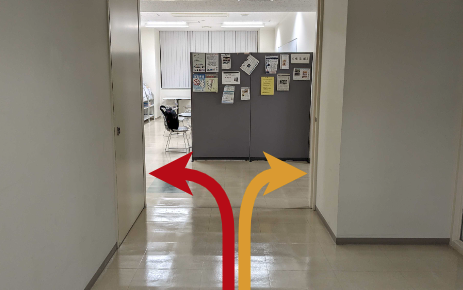
\includegraphics[height=30mm]{road.png}
  \vspace*{-4mm}
  \caption{A fork in the road where the direction of moving is not unique}
  \label{fig: fig1}
\end{figure}

\section{従来手法}
岡田らの従来手法に関して紹介する. \reffig{fig: fig2}に経路追従行動を視覚に基づいてオンラインで模倣するシステムを示す. 手法は機械学習により, 学習器の訓練を行う「学習フェーズ」と訓練した結果を検証する「テストフェーズ」に分かれる.

\subsection{学習フェーズ}
学習フェーズは, 模倣学習によって学習器の訓練を行うフェーズである. 測域センサとオドメトリを入力とする地図を用いたルールベース制御器で自律走行する. この経路追従行動を, カメラ画像を用いたend-to-endで模倣学習する. 前報\cite{okada2}で述べたように, 岡田らの手法ではデータセットの収集方法にいくつかの種類がある. 本稿では, その中で最も経路追従の成功率が高い手法を用いてロボットに模倣学習をさせる.

\subsection{テストフェーズ}
テストフェーズは, 訓練後の学習結果を評価するフェーズである. 学習器にカメラ画像を入力し, 出力されるヨー方向の角速度を用いて自律走行する.

\begin{figure}[h]
  \centering
   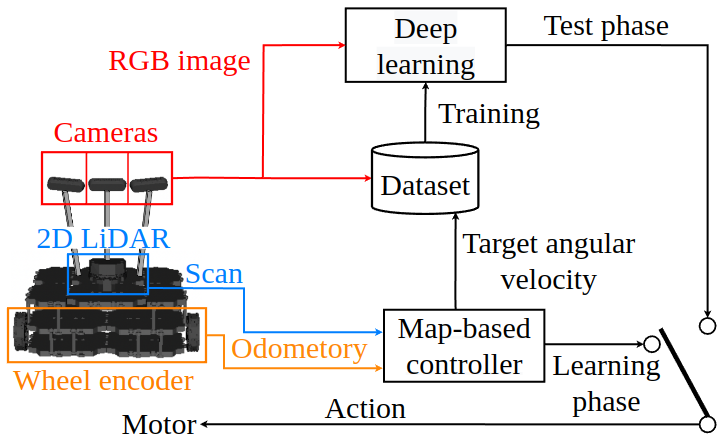
\includegraphics[width=85mm]{system.png}
   \vspace*{-4mm}
   \caption{Imitation learning system of learning phase}
   \label{fig: fig2}
 \end{figure}

\section{経路選択機能の追加}
経路選択機能の追加を目的として, データセットと学習器の入力へ, 目標とする進行方向(以下, 「目標方向」と称する)を追加する. なお, 追加した要素以外は従来手法と同様である. \reffig{fig: fig3}に提案手法のシステムを示す. 学習フェーズでは, 地図を用いたルールベース制御器で自律走行しながら, 角速度, カメラ画像に新たに目標方向をデータセットに加える. テストフェーズでは, 学習器にカメラ画像に加えて目標方向を外部から入力する. 本稿では議論しないが, 最終的に目的地までカメラ画像のみで自律走行させることを目標としているため, 目標方向を自動的に作成する仕組みが必要となる. これに関しては, カメラ画像からトポロジカルマップのどのノード上に到達したかを判定し, 目標方向を自動的に切り替えるパッケージを作成している.

\begin{figure}[h]
  \centering
   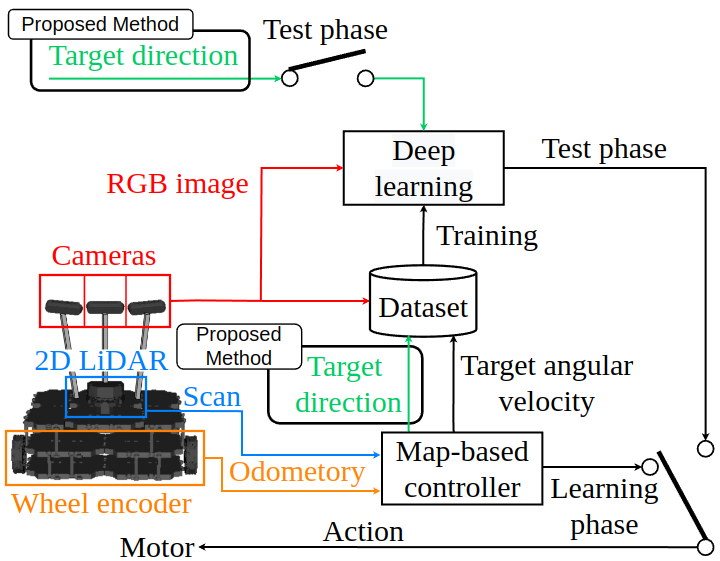
\includegraphics[width=85mm]{system2.png}
   \vspace*{-4mm}
   \caption{Imitation learning system of test phase}
   \label{fig: fig3}
 \end{figure}

\section{ネットワークとデータ形式}
\reffig{fig: fig4}に経路選択機能を追加したネットワーク, \reftab{tbl: table1}にハイパーパラメータを示す. 
先行研究に倣って, 前報で用いたネットワークの出力部へ2つの層を追加した. この層に目標方向として, \reftab{tbl: table2}のワンホットベクトルで表されるデータを入力する. なお, 文献\cite{mech}では「Continue」, 「Go straight」, 「Turn left」, 「Turn right」からなる4つのコマンドを用いていたが, 「Continue」と「Go straight」のコマンドに対応する行動がほぼ同一であったため, 本稿ではコマンドを1つ減らし, 3コマンドとしている. 
% \reffig{fig: fig5}はそれぞれの進行方向を示している.

\begin{figure}[h]
  \centering
   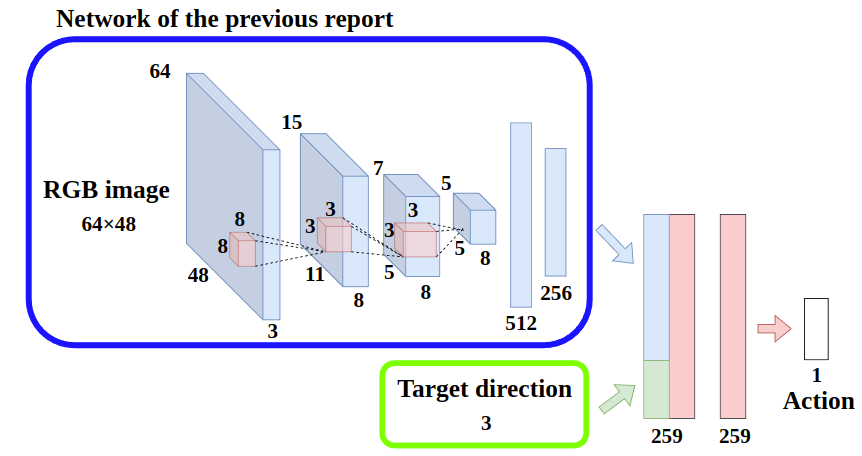
\includegraphics[width=85mm]{network.png}
   \vspace*{-4mm}
   \caption{Structure of network}
   \label{fig: fig4}
 \end{figure}

 \begin{table}[h]
  \caption{Target direction and data for imitation learning}
  \label{tbl: table1}
  \centering
  \footnotesize
  \vspace{2mm}
  \begin{tabular}{|c|c|}
   \hline
   Input data & 
   \begin{tabular}{c}
    Image (64×48 pixels, RGB channels), \\ Target direction
   \end{tabular}
   \\\hline
   Optimizer & 
   \begin{tabular}{c}
   Adam(alpha = 0.001, beta1 = 0.9, \\beta2 = 0.999, eps = 1$e^{-2}$) 
  \end{tabular}
  \\\hline 
  Loss function & Softmax-cross-entropy\\\hline
  Output data & Angular velocity\\
   \hline
  \end{tabular}
\end{table}

\begin{table}[H]
 \caption{Target direction and data for imitation learning}
 \label{tbl: table2}
 \centering
 \footnotesize
 \vspace{2mm}
 \begin{tabular}{|c|c|}
  \hline
	Target direction & Data \\\hline
  Go straight & [1, 0, 0] \\\hline
  Turn left & [0, 1, 0] \\\hline
  Turn right & [0, 0, 1] \\
  \hline
 \end{tabular}
\end{table}

% \begin{figure}[h]
%   \centering
%   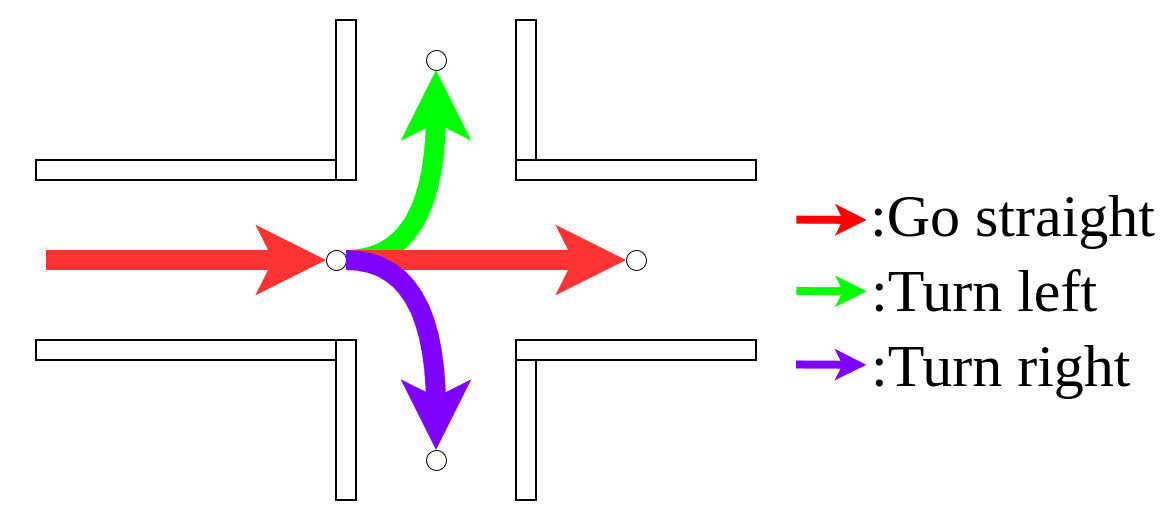
\includegraphics[width=75mm]{direction.png}
%   \vspace*{-4mm}
%   \caption{Target direction}
%   \label{fig: fig5}
% \end{figure}

% \newpage
\section{提案手法の検証実験}
文献\cite{mech}で行った実験を実環境に移して行う.
% 構築したシステムで, 目標方向に従って経路を選択できることを実環境の実験により確認する. 
\subsection{実験装置}
% \subsubsection{コンピュータ}
ロボットは, \reffig{fig: fig6}に示すような3つのカメラを搭載したロボットを用いる. また, 実験は千葉工業大学津田沼キャンパス2号館3階で行った.

\begin{figure}[h]
  \centering
   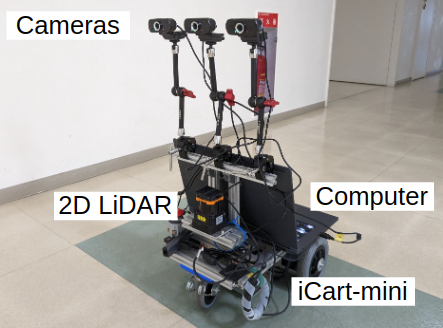
\includegraphics[width=50mm]{gamma3.png}
   \vspace*{-4mm}
   \caption{Experimental setup}
   \label{fig: fig6}
 \end{figure}

 \subsection{実験方法}
 \reffig{fig: fig7}に示すような A,B の三叉路で全ての侵入方向と抜け出す経路を含めるように, 文献\cite{mech}と同様の経路を繰り返し走行させる. 学習を60000step実行後, テストフェーズに移行する. テストフェーズでは, 学習フェーズと同様の経路を, 目標方向による制御によって正しく走行できるか評価する.

 \begin{figure}[h]
  \centering
   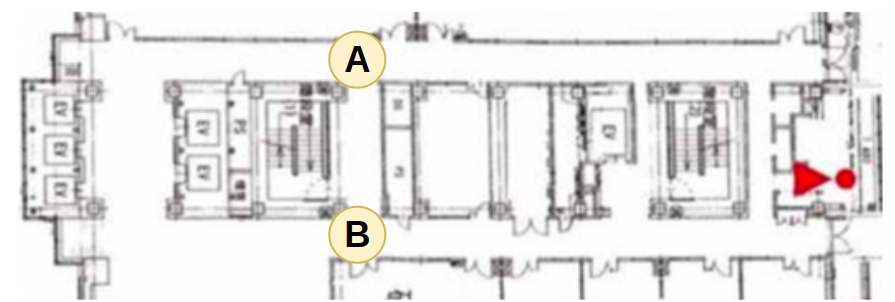
\includegraphics[width=70mm]{tsudanuma2.png}
   \vspace*{-4mm}
   \caption{Experimental environment}
   \label{fig: fig7}
 \end{figure}


% 本文:明朝体・9pt(欧文Times New Roman, 9pt)、文字間隔は1行26文字程度、行間隔は4.2mm程度にして下さ	い。

% \subsection{論文作成に関する注意事項を以下に示します。(中見出し:ゴシック体・9pt・強調文字・左寄せ)}%-----------
% \begin{itemize}
% 	\item 用紙サイズ:A4(210×297mm)とします。
% 	\item 用紙マージン:上下25mm。日本語表題から\textbf{\textit{Key Words}}までの1段組の部分は、左右25mm以上空けて下さい。本文からは2段組とし、左右15mm、段間は6mmとします。
% 	\item 文字のフォント、大きさ:\reftab{tbl: table1}を参照下さい。
% 	\item 図の画質:300dpi以上の画質の高いものにして下さい。
% 	\item 図・表のタイトル:図のタイトルには「Fig.\# English title」、表のタイトルには「Table \# English title」という形式を用い、文中ではそれぞれ「図\#」、「表\#」という表現にして下さい。
% 	\item グラフの軸タイトル:各軸のタイトルに変数記号だけを記述するのは避けて下さい。\reffig{fig: fig1}に示すように、軸を表す語句ならびに単位を記入して下さい。
% 	\item 式:以下に示すように、右寄せで番号をふり、式は中央に配置して下さい。文中では「\refeqn{eqn: eq1}」と表現して下さい。
	
% 	\begin{equation}
% 		M\ddot{r}_{str1} + F_{frk} = Mg
% 		\label{eqn: eq1}
% 	\end{equation}

% 	\item 単位:SI単位系とします。
% 	\item 本文中に文献を引用する場合、引用を表す語句や文の後ろに文献番号(例えば\cite{Shinjuku98})を振って下さい。文献を主語や目的語などに用いる場合、「文献\cite{Shinjuku98}では、・・」などのようにして、番号のみの表現を避けて下さい。
% 	\item 連名の場合には講演発表者氏名の前に○印をつけて下さい。
% 	\item 作成した論文はPDFファイル形式に変換し、PDFファイルのみを学会本部へ提出して下さい。PDFファイルの提出は本講演会ホームページ記載のアップロードのページの指示に従って下さい。
% 	\item[]
% 	\item[※] ただし、PDFファイルの容量は2MB以下、論文のページ数は2頁以上4頁以下とします。なお、印刷原稿の提出は不要ですので、郵送しないで下さい。
% 	\item[※] 講演番号、講演会名、ページ番号は記載しないようにして下さい。
% \end{itemize}

% %※ ただし、PDFファイルの容量は2MB以下、論文のページ数は2頁以上4頁以下とします。なお、印刷原稿の提出は不要ですので、郵送しないで下さい。

% %※ 講演番号、講演会名、ページ番号は記載しないようにして下さい。


% \begin{table}[h]
%  \caption{Type size and typefaces for papers}
%  \label{tbl: table1}
%  \centering
%  \footnotesize
%  \begin{tabular}{|p{7zw}|c|c|c|}
%   \hline
% 	適用場所	&日本語	&欧文 \\\hline
% 	標準のフォント	&明朝体 9pt	&Times New Roman 9pt \\\hline
% 	日本語表題	&ゴシック体 14pt	&Arial 14pt \\\hline
% 	日本語副表題	&ゴシック体 12pt	&Arial 12pt \\\hline
% 	英語表題	&-&Times New Roman 12pt \\\hline
% 	英語副表題	&-&Times New Roman 10pt \\\hline
% 	日本語著者名	&明朝体 10pt &-\\\hline
% 	英語著者名	&-&Times New Roman 9pt \\\hline
% 	アブストラクト・キーワード	&-&Times New Roman 9pt \\\hline
% 	大見出し	&ゴシック体 10pt	&Arial 10pt \\\hline
% 	中見出し	&ゴシック体 9pt	&Arial 9pt \\\hline
% 	図・表の番号・タイトル	 &-&Times New Roman 9pt \\\hline
% 	文献	&明朝体 8pt	&Times New Roman 8pt \\
%   \hline
%  \end{tabular}
% \end{table}

% \begin{figure}[h]
%  \centering
%   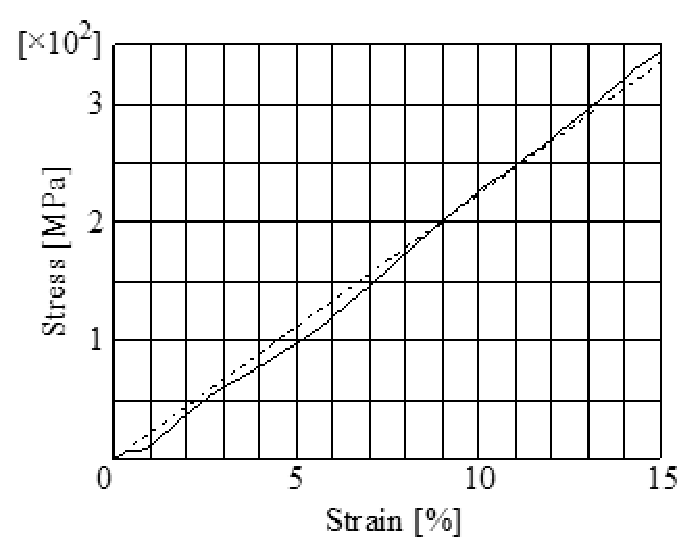
\includegraphics[height=38mm]{fig1.eps}
%   \vspace*{-4mm}
%   \caption{Tensile stress-strain diagram}
%   \label{fig: fig1}
% \end{figure}


\footnotesize
\begin{thebibliography}{99}

% \bibitem{Shinjuku98}
% 新宿大五朗,渋谷次郎,東京 学,``キャスティングマニピュレーションに関する研究(第1報,可変長の紐状柔軟リンクを有するマニピュレータの提案とそのスイング制御法)'',{\it 機論C編}, vol.64-626, pp.3854--3861, 1998.

% \bibitem{Shinjuku99}
% Shinjuku, D., Shibuya, J. and Tokyo, M., ``Swing Motion Control of Casting Manipulation,'' {\it IEEE Control Systems}, vol.19-4, pp.56--64, 1999.

\bibitem{okada1}
岡田眞也,清岡優祐, 上田隆一,林原靖男“視覚と行動の : end-to-end 学習により経路追従行動 をオンラインで模倣する手法の提案”,計測自動制御学会 SI 部門講演会 SICE-SI2020 予稿集,pp.1147–1152(2020)

\bibitem{okada2}
岡田眞也,清岡優祐,春山健太,上田隆一,林原靖男:“視覚と 行動の end-to-end 学習により経路追従行動 をオンラインで 模倣する手法の提案 -経路追従行動の修正のためにデータセッ トを動的に追加する手法の検討”,計測自動制御学会 SI 部門 講演会 SICE-SI2021 予稿集,pp.1066-1070(2021)

\bibitem{bojarski}
Bojarski, Mariusz,et al. “End to end learning for self- driving cars.”arXiv:1604.07316(2016)

\bibitem{moridian}
Moridian, Barzin, Anurag Kamal, and Nina Mahmoudian. "Learning navigation tasks from demonstration for semi- autonomous remote operation of mobile robots." 2018 IEEE International Symposium on Safety, Security, and Rescue Robotics (SSRR). IEEE, (2018)

\bibitem{felipe}
Felipe Codevilla et al.“end-to-end driving via conditional imitation learning.” arXiv: 1710.02410(2018)

\bibitem{mech}
春山健太, 藤原柾, 清岡優祐, 岡田眞也, 上田隆一, 林原靖男,“視覚と行動の end-to-end 学 習により経路追従行動をオンラインで模倣する手法の提案―経路選択機能の追加―“, 日 本機械学会ロボティクス・メカトロニクス講演会’22 予稿集,(2022).

\bibitem{hawke}
Jeffrey hawke et al. ”urban driving with conditional imitation learning”. arxiv: 1912.00177, 2019.

\bibitem{nav}
ros-planning, navigation レポジトリ. \url{https://github.com/ros-planning/navigation.}

\bibitem{waypoint}
waypoint\_nav レポジトリ. \url{https://github.com/open-rdc/waypoint_nav.git.}

\end{thebibliography}

\normalsize
\end{document}
